\documentclass[tikz,border=3pt]{standalone}
% Shared preamble for the standalone TikZ diagrams (included after \documentclass).
% Build with build.sh. Language is selected with \def\VI{1} (Vietnamese) or by default English:
%   \LL{English text}{Văn bản tiếng Việt}
\usepackage{fontspec}
\IfFontExistsTF{Times New Roman}{\setmainfont{Times New Roman}}{%
  \setmainfont{times.ttf}[Path=/mnt/c/Windows/Fonts/,
    BoldFont=timesbd.ttf,ItalicFont=timesi.ttf,BoldItalicFont=timesbi.ttf]}
\usepackage{xcolor}
\usepackage{tikz}
\usetikzlibrary{arrows.meta,positioning,calc,fit,backgrounds,patterns,shapes.misc,decorations.pathreplacing}

\newcommand{\LL}[2]{\ifdefined\VI #2\else #1\fi}
\hyphenpenalty=10000 \exhyphenpenalty=10000 \tolerance=9999 \emergencystretch=3em

% --- palette (print-safe: meaning is never carried by colour alone) -----------
\definecolor{ink}{HTML}{1F2937}
\definecolor{muted}{HTML}{6B7280}
\definecolor{rule}{HTML}{9CA3AF}
\definecolor{shfill}{HTML}{DCE8F5}   % shared
\definecolor{shline}{HTML}{2F5D8C}
\definecolor{dedfill}{HTML}{FBE5CF}  % dedicated
\definecolor{dedline}{HTML}{B5651D}
\definecolor{neutral}{HTML}{F3F4F6}
\definecolor{appfill}{HTML}{F6F9FC}
\definecolor{appline}{HTML}{7C93AD}
\definecolor{ctlfill}{HTML}{EFEAF7}
\definecolor{ctlline}{HTML}{6B5B95}
\definecolor{warn}{HTML}{B91C1C}
\definecolor{ta}{HTML}{2A9D8F}       % tenant A
\definecolor{tb}{HTML}{E09F3E}       % tenant B
\definecolor{tc}{HTML}{8E6BBF}       % tenant C
\colorlet{taL}{ta!22}
\colorlet{tbL}{tb!28}
\colorlet{tcL}{tc!24}

\tikzset{
  >=Latex,
  every node/.style={font=\footnotesize, text=ink, inner sep=2pt},
  box/.style={draw=ink!65, rounded corners=1.6pt, line width=0.5pt, fill=white,
              align=center, inner sep=3pt, minimum height=5mm},
  shared/.style={box, fill=shfill, draw=shline},
  ded/.style={box, fill=dedfill, draw=dedline},
  plain/.style={box, fill=neutral, draw=rule},
  ta/.style={box, fill=taL, draw=ta},
  tb/.style={box, fill=tbL, draw=tb},
  tc/.style={box, fill=tcL, draw=tc},
  tenantA/.style={ta}, tenantB/.style={tb}, tenantC/.style={tc},
  zone/.style={draw=appline, fill=appfill, rounded corners=2.5pt, line width=0.6pt},
  ctlzone/.style={draw=ctlline, fill=ctlfill, rounded corners=2.5pt, line width=0.6pt},
  ttl/.style={font=\small\bfseries, text=ink, align=left, inner sep=1pt},
  cp/.style={font=\scriptsize, text=muted, align=center, inner sep=1pt},
  note/.style={font=\scriptsize, text=muted, align=left, inner sep=1pt},
  arr/.style={->, line width=0.6pt, draw=ink!80},
  arrm/.style={->, line width=0.6pt, draw=muted, dashed},
  link/.style={line width=0.5pt, draw=muted},
  bound/.style={line width=0.8pt, draw=warn, dash pattern=on 3pt off 2pt},
  badge/.style={circle, fill=ink, text=white, font=\scriptsize\bfseries, inner sep=1.2pt, minimum size=3.6mm},
}

% a small user glyph (head + shoulders) centred at the given coordinate, colour as 3rd arg

% user glyph: head and shoulders, centred at (x,y); 3rd argument = colour
\newcommand{\user}[3]{%
  \fill[#3] (#1,#2) circle (0.85mm);
  \fill[#3] ($(#1,#2)+(-1.5mm,-2.5mm)$) arc (180:0:1.5mm) -- cycle;}

% Figure: scenario space. Rows = layers of the modern stack; columns = scenarios; colour = shared / dedicated.
% Scenarios S1-S4 keep every satellite layer identical, so that differences are caused by the data layer alone.
\begin{document}
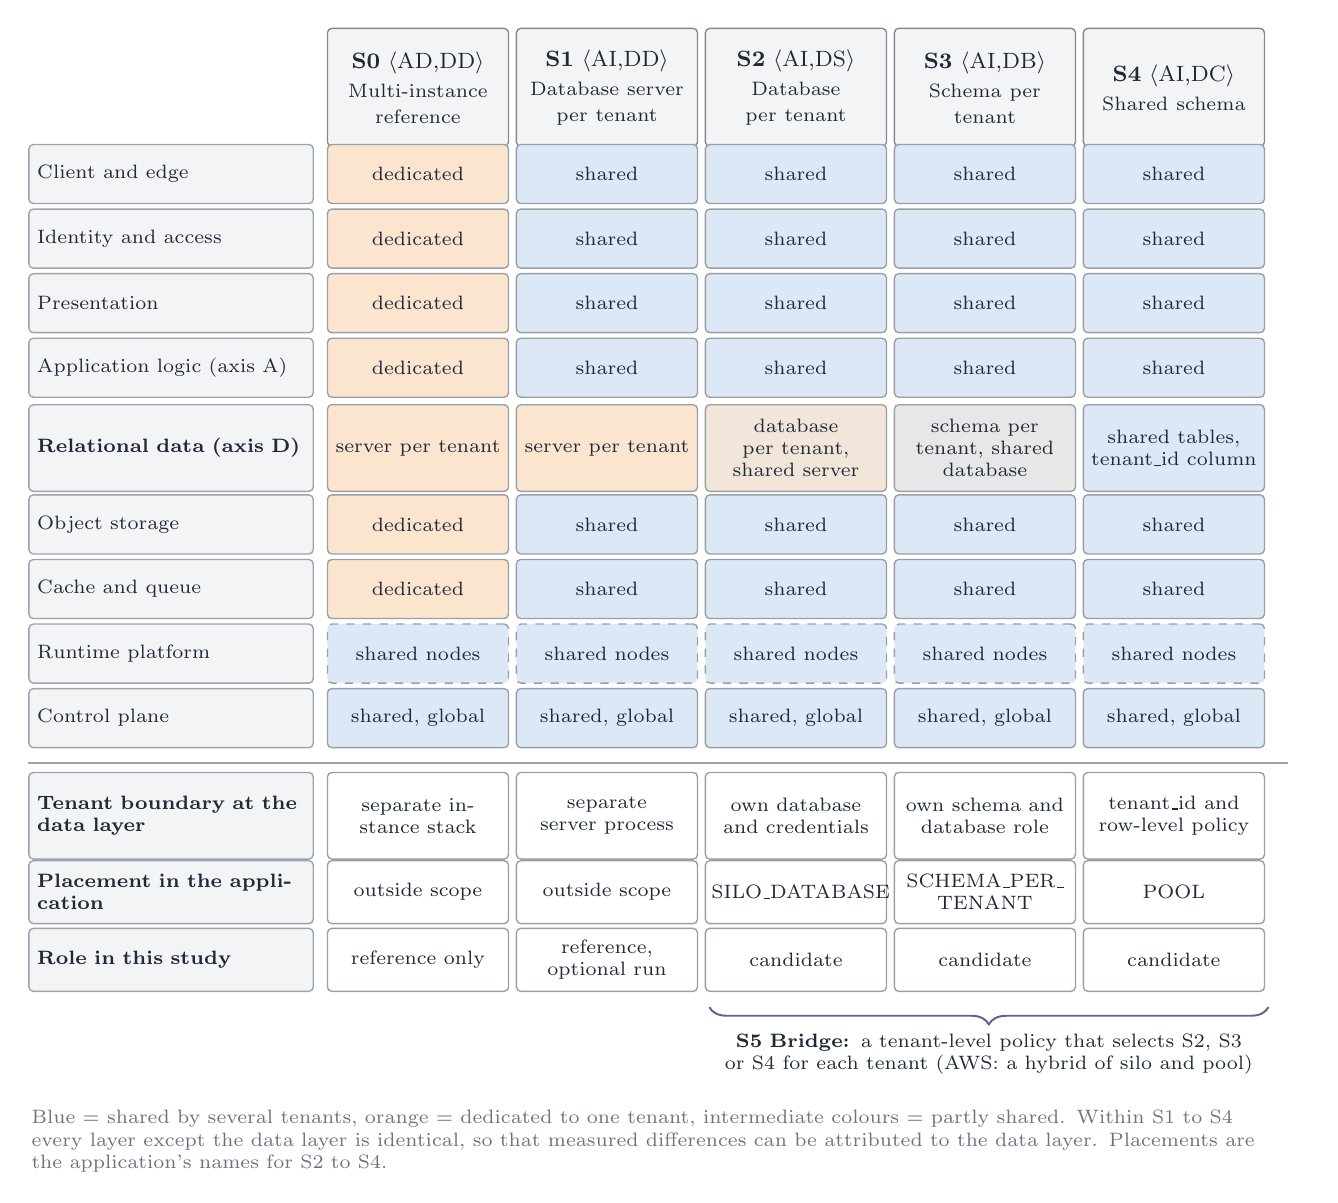
\begin{tikzpicture}[x=1mm,y=1mm]
\colorlet{g1}{shfill}
\colorlet{g2}{shfill!62!dedfill}
\colorlet{g3}{shfill!30!dedfill}
\colorlet{g4}{dedfill}

% cell(column index, y centre, height, fill, text)
\newcommand{\cell}[5]{\node[box,fill=#4,draw=ink!45,minimum width=23mm,minimum height=#3mm,text width=21.5mm,font=\scriptsize,inner sep=1pt] at (49.5+#1*24,#2) {#5};}
\newcommand{\rowlabel}[4]{\node[plain,minimum width=36mm,minimum height=#3mm,text width=34mm,align=left,anchor=west,font=\scriptsize,inner sep=3pt] at (0,#2) {#4};}

% ------------------------------------------------------------------ column headers
\foreach \i/\id/\tup/\en/\vi in {
  0/S0/{$\langle$AD,DD$\rangle$}/{Multi-instance reference}/{Tham chiếu đa thể hiện},
  1/S1/{$\langle$AI,DD$\rangle$}/{Database server per tenant}/{Máy chủ CSDL riêng mỗi thuê bao},
  2/S2/{$\langle$AI,DS$\rangle$}/{Database per tenant}/{CSDL riêng mỗi thuê bao},
  3/S3/{$\langle$AI,DB$\rangle$}/{Schema per tenant}/{Lược đồ riêng mỗi thuê bao},
  4/S4/{$\langle$AI,DC$\rangle$}/{Shared schema}/{Lược đồ dùng chung}} {
  \node[box,fill=neutral,draw=ink!55,minimum width=23mm,minimum height=15mm,text width=21.5mm,inner sep=1.5pt] at (49.5+\i*24,110) {\textbf{\id}\ \tup\\[1pt]{\scriptsize\LL{\en}{\vi}}};
}

% ------------------------------------------------------------------ rows (layers)
\rowlabel{}{99}{7.5}{\LL{Client and edge}{Máy khách và biên}}
\rowlabel{}{90.8}{7.5}{\LL{Identity and access}{Định danh và truy cập}}
\rowlabel{}{82.6}{7.5}{\LL{Presentation}{Trình diễn}}
\rowlabel{}{74.4}{7.5}{\LL{Application logic (axis A)}{Logic ứng dụng (trục A)}}
\rowlabel{}{64.2}{11}{\textbf{\LL{Relational data (axis D)}{Dữ liệu quan hệ (trục D)}}}
\rowlabel{}{54.5}{7.5}{\LL{Object storage}{Lưu trữ đối tượng}}
\rowlabel{}{46.3}{7.5}{\LL{Cache and queue}{Bộ nhớ đệm và hàng đợi}}
\rowlabel{}{38.1}{7.5}{\LL{Runtime platform}{Nền tảng thực thi}}
\rowlabel{}{29.9}{7.5}{\LL{Control plane}{Mặt phẳng điều khiển}}

\foreach \y/\h in {99/7.5,90.8/7.5,82.6/7.5,74.4/7.5,54.5/7.5,46.3/7.5} {
  \cell{0}{\y}{\h}{g4}{\LL{dedicated}{riêng}}
  \foreach \c in {1,2,3,4} { \cell{\c}{\y}{\h}{g1}{\LL{shared}{dùng chung}} }
}
% relational data row
\cell{0}{64.2}{11}{g4}{\LL{server per tenant}{máy chủ riêng}}
\cell{1}{64.2}{11}{g4}{\LL{server per tenant}{máy chủ riêng}}
\cell{2}{64.2}{11}{g3}{\LL{database per tenant, shared server}{CSDL riêng, máy chủ chung}}
\cell{3}{64.2}{11}{g2}{\LL{schema per tenant, shared database}{lược đồ riêng, CSDL chung}}
\cell{4}{64.2}{11}{g1}{\LL{shared tables, tenant\_id column}{bảng dùng chung, cột tenant\_id}}
% runtime and control plane rows (same in every scenario)
\foreach \c in {0,1,2,3,4} {
  \node[box,dashed,fill=g1,draw=ink!45,minimum width=23mm,minimum height=7.5mm,text width=21.5mm,font=\scriptsize,inner sep=1pt] at (49.5+\c*24,38.1) {\LL{shared nodes}{nút dùng chung}};
  \cell{\c}{29.9}{7.5}{g1}{\LL{shared, global}{dùng chung, toàn cục}}
}

% ------------------------------------------------------------------ text rows
\draw[rule,line width=0.4pt] (0,24.2) -- (160,24.2);
\rowlabel{}{17.5}{11}{\textbf{\LL{Tenant boundary at the data layer}{Ranh giới thuê bao ở tầng dữ liệu}}}
\rowlabel{}{7.8}{8}{\textbf{\LL{Placement in the application}{Vị trí dữ liệu trong ứng dụng}}}
\rowlabel{}{-0.8}{8}{\textbf{\LL{Role in this study}{Vai trò trong nghiên cứu}}}
\foreach \i/\en/\vi/\pen/\pvi/\ren/\rvi in {
  0/{separate instance stack}/{bộ thể hiện riêng}/{outside scope}/{ngoài phạm vi}/{reference only}/{chỉ để tham chiếu},
  1/{separate server process}/{tiến trình máy chủ riêng}/{outside scope}/{ngoài phạm vi}/{reference, optional run}/{tham chiếu, chạy tùy chọn},
  2/{own database and credentials}/{CSDL và thông tin đăng nhập riêng}/{SILO\_DATABASE}/{SILO\_DATABASE}/{candidate}/{ứng viên},
  3/{own schema and database role}/{lược đồ và role CSDL riêng}/{SCHEMA\_PER\_\allowbreak TENANT}/{SCHEMA\_PER\_\allowbreak TENANT}/{candidate}/{ứng viên},
  4/{tenant\_id and row-level policy}/{tenant\_id và chính sách mức dòng}/{POOL}/{POOL}/{candidate}/{ứng viên}} {
  \node[box,fill=white,draw=ink!45,minimum width=23mm,minimum height=11mm,text width=21.5mm,font=\scriptsize,inner sep=1pt] at (49.5+\i*24,17.5) {\LL{\en}{\vi}};
  \node[box,fill=white,draw=ink!45,minimum width=23mm,minimum height=8mm,text width=21.5mm,font=\scriptsize,inner sep=1pt] at (49.5+\i*24,7.8) {\LL{\pen}{\pvi}};
  \node[box,fill=white,draw=ink!45,minimum width=23mm,minimum height=8mm,text width=21.5mm,font=\scriptsize,inner sep=1pt] at (49.5+\i*24,-0.8) {\LL{\ren}{\rvi}};
}

% ------------------------------------------------------------------ S5 bridge brace
\draw[decorate,decoration={brace,mirror,amplitude=2.2mm},line width=0.7pt,draw=ctlline] (86.5,-6.8) -- node[below=2.6mm,font=\scriptsize,text=ink,text width=80mm,align=center] {\textbf{S5 Bridge:} \LL{a tenant-level policy that selects S2, S3 or S4 for each tenant (AWS: a hybrid of silo and pool)}{chính sách theo thuê bao chọn S2, S3 hoặc S4 cho từng thuê bao (AWS: lai giữa silo và pool)}} (157.5,-6.8);

\node[note,anchor=north west,text width=158mm] at (0,-19.5) {\LL{Blue = shared by several tenants, orange = dedicated to one tenant, intermediate colours = partly shared. Within S1 to S4 every layer except the data layer is identical, so that measured differences can be attributed to the data layer. Placements are the application's names for S2 to S4.}{Xanh dương = dùng chung nhiều thuê bao, cam = dành riêng cho một thuê bao, màu trung gian = chia sẻ một phần. Trong S1 đến S4 mọi tầng ngoài tầng dữ liệu đều giống nhau, để chênh lệch đo được quy cho tầng dữ liệu. Tên vị trí là tên mà ứng dụng dùng cho S2 đến S4.}};

\end{tikzpicture}
\end{document}
